\documentclass[12pt,a4paper]{article}
\usepackage{ctex}
\usepackage{amsmath,amscd,amsbsy,amssymb,latexsym,url,bm,amsthm}
\usepackage{epsfig,graphicx,subfigure}
\usepackage{enumitem,balance}
\usepackage{wrapfig}
\usepackage{mathrsfs,euscript}
\usepackage[usenames]{xcolor}
\usepackage{hyperref}
\usepackage[vlined,ruled,linesnumbered]{algorithm2e}
\usepackage{float}
\usepackage{multirow}

\hypersetup{colorlinks=true,linkcolor=blue}

\newtheorem{theorem}{Theorem}
\newtheorem{lemma}[theorem]{Lemma}
\newtheorem{proposition}[theorem]{Proposition}
\newtheorem{corollary}[theorem]{Corollary}
\newtheorem{exercise}{Exercise}
\newtheorem*{solution}{Solution}
\newtheorem{definition}{Definition}
\theoremstyle{definition}



\renewcommand{\thefootnote}{\fnsymbol{footnote}}

\newcommand{\postscript}[2]
 {\setlength{\epsfxsize}{#2\hsize}
  \centerline{\epsfbox{#1}}}

\renewcommand{\baselinestretch}{1.0}

\setlength{\oddsidemargin}{-0.365in}
\setlength{\evensidemargin}{-0.365in}
\setlength{\topmargin}{-0.3in}
\setlength{\headheight}{0in}
\setlength{\headsep}{0in}
\setlength{\textheight}{10.1in}
\setlength{\textwidth}{7in}
\makeatletter \renewenvironment{proof}[1][Proof] {\par\pushQED{\qed}\normalfont\topsep6\p@\@plus6\p@\relax\trivlist\item[\hskip\labelsep\bfseries#1\@addpunct{.}]\ignorespaces}{\popQED\endtrivlist\@endpefalse} \makeatother
\makeatletter
\renewenvironment{solution}[1][Solution] {\par\pushQED{\qed}\normalfont\topsep6\p@\@plus6\p@\relax\trivlist\item[\hskip\labelsep\bfseries#1\@addpunct{.}]\ignorespaces}{\popQED\endtrivlist\@endpefalse} \makeatother

\begin{document}
\noindent

%========================================================================
\noindent\framebox[\linewidth]{\shortstack[c]{
\Large{\textbf{Lab10-Turing Machine}}\vspace{1mm}\\
Algorithm and Complexity (CS214), Xiaofeng Gao, Spring 2020.}}
\begin{center}
\footnotesize{\color{red}$*$ If there is any problem, please contact TA Yiming Liu. }

\footnotesize{\color{blue}$*$ Name:HanzhangYang  \quad Student ID:518030910022 \quad Email: linqinluli@sjtu.edu.cn}
\end{center}

\begin{enumerate}

\item
Design a one-tape TM $M$ that computes the function $f(x, y) = x \mod y$, where $x$ and $y$ are positive integers ($x > y$). The alphabet is $\{1, 0, \Box, \triangleright, \triangleleft\}$, and the inputs are $x$ 1's, $\Box$ and $y$ 1's. Below is the initial configuration for input $x=7$ and $y=3$. The result $z=f(x, y)$ should also be represented in the form of $z$ 1's on the tape with the pattern of $\triangleright 111 \cdots 111 \triangleleft$.
\begin{center}
	\begin{tabular}{ll|c|c|c|c|c|c|c|c|c|c|c|c|c|c}
		& \multicolumn{14}{c}{Initial Configuration}\\[5pt]
		\cline{2-16}
		& & $\triangleright$ &  1  & 1 & 1 & 1 & 1 & 1 & 1 & $\Box$ & 1 & 1 & 1 & $ \triangleleft$ & \\
		\cline{2-16}
		\multicolumn{2}{c}{} & \multicolumn{1}{c}{$\uparrow$} & \multicolumn{11}{c}{}\\[-4px]
		\multicolumn{2}{c}{} & \multicolumn{1}{c}{$q_S$} & \multicolumn{11}{c}{}	
	\end{tabular}
\end{center}

\begin{enumerate}
	\item
	Please describe your design and then write the specifications of $M$ in the form like $\langle q_S, \triangleright \rangle \rightarrow \langle q_1, \triangleright,  R\rangle$. Explain the transition functions in detail.
	
	\item
	Please draw the state transition diagram.
	
	\item
	Show briefly and clearly the whole process from initial to final configurations for input $x = 7$ and $y = 3$. You may start like this:
	$$(q_s,\underline{\triangleright}  1  1  1  1  1  1  1  \Box 1  1  1   \triangleleft)
	\vdash (q_1,\triangleright  \underline{1}  1  1  1  1  1  1  \Box 1  1  1   \triangleleft)
	\vdash^* (q_1,\triangleright  1  1  1  1  1  1  1  \underline{\Box} 1  1  1   \triangleleft)
	\vdash (q_2,\triangleright  1  1  1  1  1  1  1  \Box \underline{1}  1  1   \triangleleft)$$
	
	\par{\color{blue}(Note that for simplicity, we write $(q_1,\triangleright  \underline{1}  1  1  1  1  1  1  \Box 1  1  1   \triangleleft)\vdash^* (q_1,\triangleright  1  1  1  1  1  1  1  \underline{\Box} 1  1  1   \triangleleft)$ if the corresponding transaction repeats on multiple inputs with the same state.)}
	
\end{enumerate}

\textbf{Solution.}

(a) For every loop, change 1 to 0 of y one by one. At the same time, change the 1 of x whith the exchange of y. After all 1 of y have been changed, change all 0 in y to 1.

Finally, all 1 in x have been changed and the answer is stored in y.

$\langle q_S, \triangleright \rangle \rightarrow \langle q_1, \triangleright,  R\rangle$\\
$\langle q_1,  1\rangle \rightarrow \langle q_1, 1,  R\rangle$\qquad(move to y)\\
$\langle q_1,  \Box\rangle \rightarrow \langle q_2, \Box,  R\rangle$\qquad(change to $q_2$)\\
$\langle q_2,  0\rangle \rightarrow \langle q_2, 0,  R\rangle$\qquad(move to the first 1)\\
$\langle q_2,  \Box\rangle \rightarrow \langle q_2, \Box,  R\rangle$\qquad(move to the first 1)\\
$\langle q_2,  1\rangle \rightarrow \langle q_3, 0,  L\rangle$\qquad(change the first 1 to 0)\\
$\langle q_2,  \triangleleft\rangle \rightarrow \langle q_4, \triangleleft,  L\rangle$\qquad(no 1 left, change to $q_4$)\\
$\langle q_4,  0\rangle \rightarrow \langle q_4, 1,  L\rangle$\qquad(change all 0 in y to 1 again)\\
$\langle q_4,  \Box\rangle \rightarrow \langle q_2, \Box,  R\rangle$\qquad(change to $q_2$ again)\\
$\langle q_3,  1\rangle \rightarrow \langle q_2, \Box,  R\rangle$\qquad(change 1 in x to $\Box$)\\
$\langle q_3,  \Box\rangle \rightarrow \langle q_3, \Box,  L\rangle$\qquad(move to the last 1 in x)\\
$\langle q_3,  0\rangle \rightarrow \langle q_3, 0,  L\rangle$\qquad(move to the last 1 in x)\\
$\langle q_3,  \triangleright\rangle \rightarrow \langle q_5, \Box,  R\rangle$\qquad(all 1 in x have been changed)\\
$\langle q_5,  \Box\rangle \rightarrow \langle q_5, \Box,  R\rangle$\qquad(move to get the answer)\\
$\langle q_5,  0\rangle \rightarrow \langle q_6, \triangleright,  R\rangle$\qquad(clear the first 0)\\
$\langle q_6,  0\rangle \rightarrow \langle q_6, 1,  R\rangle$\qquad(set answer)\\
$\langle q_6,  1\rangle \rightarrow \langle q_7, \triangleleft,  R\rangle$\qquad(answer have been set, clear the rest symble)\\
$\langle q_7,  1\rangle \rightarrow \langle q_7, \Box,  R\rangle$\qquad(clear)\\
$\langle q_7,  \triangleleft\rangle \rightarrow \langle q_H, \Box,  S\rangle$\qquad(get the final answer)\\

(b)\textbf{State Transition Diagram}
\begin{figure}[H] 
    \centering 
    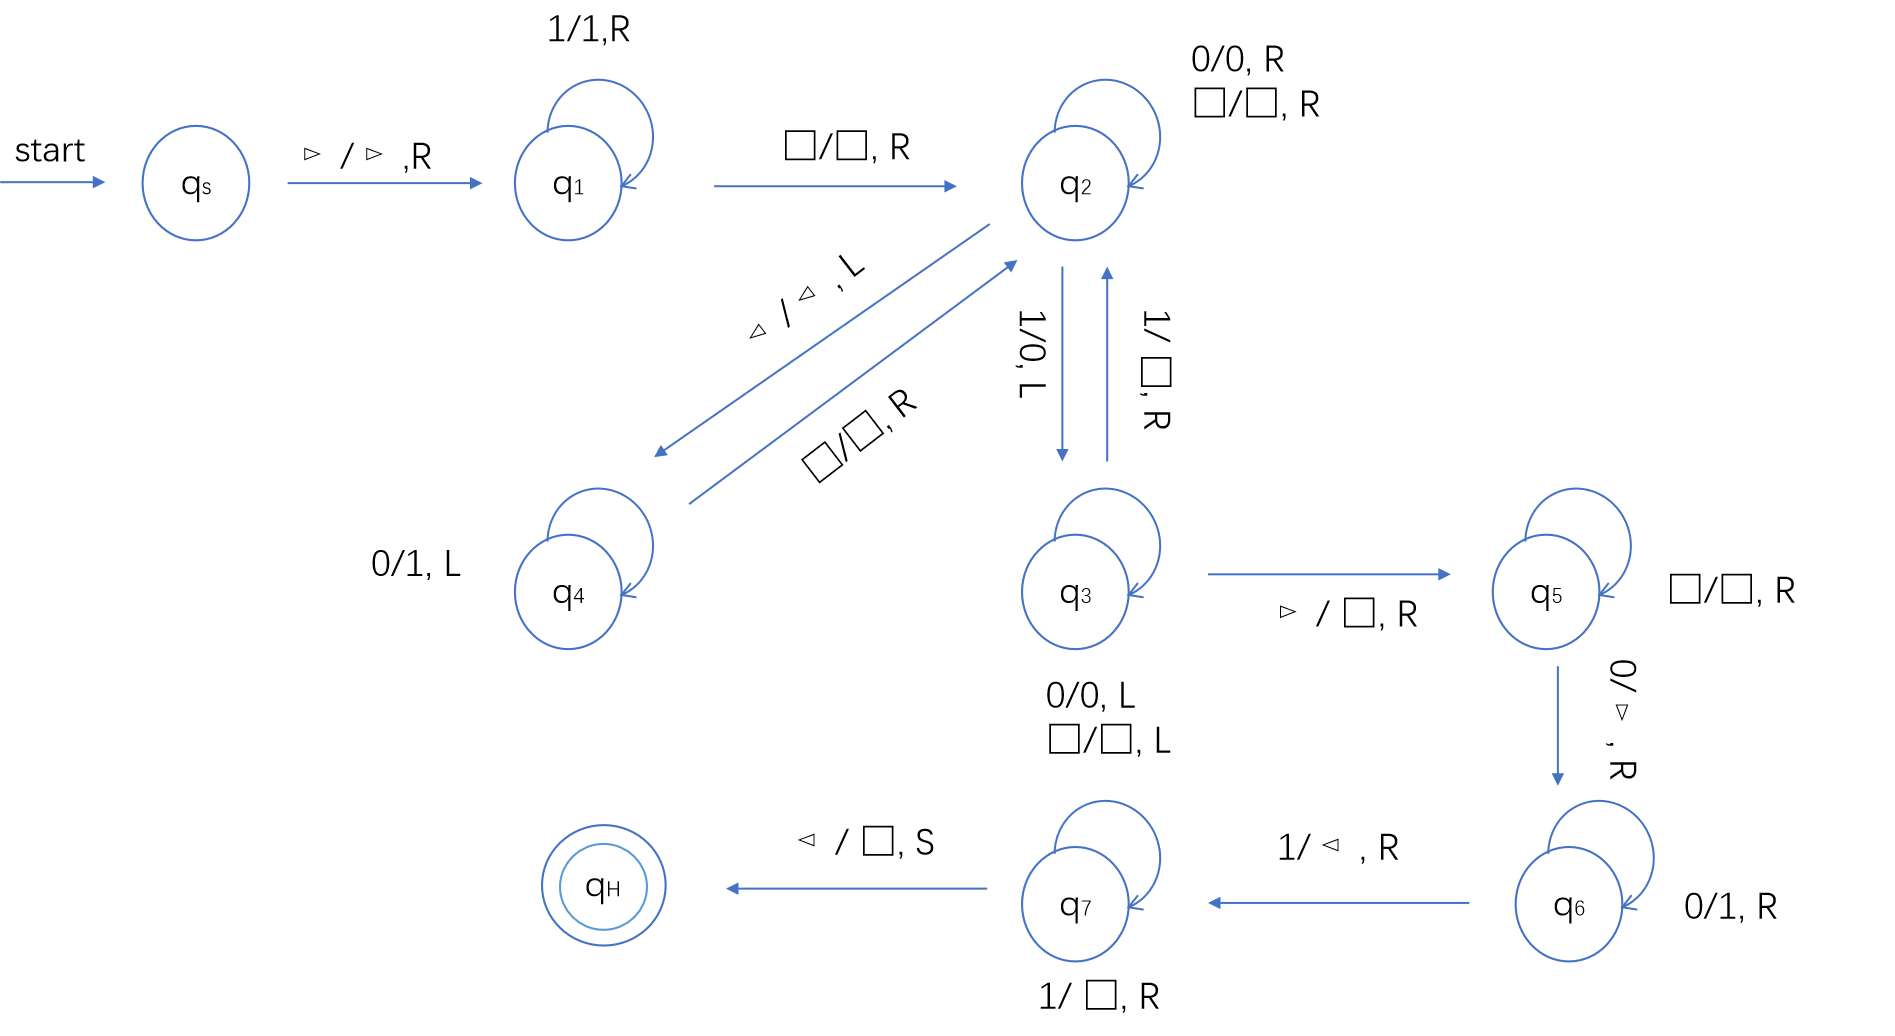
\includegraphics[width=0.9\textwidth]{2} 

\end{figure}
(c)
$$(q_s,\underline{\triangleright}  1  1  1  1  1  1  1  \Box 1  1  1   \triangleleft)
\vdash (q_1,\triangleright  \underline{1}  1  1  1  1  1  1  \Box 1  1  1   \triangleleft)
\vdash^* (q_1,\triangleright  1  1  1  1  1  1  1  \underline{\Box} 1  1  1   \triangleleft)$$
$$\vdash (q_2,\triangleright  1  1  1  1  1  1  1  \Box \underline{1}  1  1   \triangleleft)
\vdash (q_3,\triangleright  1  1  1  1  1  1  1  \underline{\Box} 0  1  1   \triangleleft)
\vdash (q_3,\triangleright  1  1  1  1  1  1  \underline{1}  \Box 0  1  1   \triangleleft)$$
$$\vdash (q_2,\triangleright  1  1  1  1  1  1  \Box  \Box \underline{0}  1  1   \triangleleft)
\vdash (q_2,\triangleright  1  1  1  1  1  1  \Box  \Box 0  \underline{1}  1   \triangleleft)
\vdash (q_3,\triangleright  1  1  1  1  1  1  \Box  \Box \underline{0}  0  1   \triangleleft)$$
$$\vdash^* (q_3,\triangleright  1  1  1  1  1  \underline{1}  \Box  \Box 0  0  1   \triangleleft)
\vdash (q_2,\triangleright  1  1  1  1  1  \Box  \underline{\Box}  \Box 0  0  1   \triangleleft)
\vdash^* (q_2,\triangleright  1  1  1  1  1  \Box  \Box  \Box 0  0  \underline{1}   \triangleleft)$$
$$\vdash (q_3,\triangleright  1  1  1  1  1  \Box  \Box  \Box 0  \underline{0}  0   \triangleleft)
\vdash^* (q_3,\triangleright  1  1  1  1  \underline{1}  \Box  \Box  \Box 0  0  0   \triangleleft)
\vdash (q_2,\triangleright  1  1  1  1  \Box  \underline{\Box}  \Box  \Box 0  0  0   \triangleleft)$$
$$\vdash^* (q_2,\triangleright  1  1  1  1  \Box  \Box  \Box  \Box 0  0  0   \underline{\triangleleft})
\vdash (q_4,\triangleright  1  1  1  1  \Box  \Box  \Box  \Box 0  0  \underline{0}   \triangleleft)
\vdash^* (q_4,\triangleright  1  1  1  1  \Box  \Box  \Box  \underline{\Box} 1  1  1   \triangleleft)$$
$$\vdash (q_2,\triangleright  1  1  1  1  \Box  \Box  \Box  \Box \underline{1}  1  1   \triangleleft)
\vdash (q_3,\triangleright  1  1  1  1  \Box  \Box  \Box  \Box \underline{0}  1  1   \triangleleft)
\vdash^* (q_3,\triangleright  1  1  1  \underline{1}  \Box  \Box  \Box  \Box 0  1  1   \triangleleft)$$
$$\vdash (q_2,\triangleright  1  1  1  \Box  \underline{\Box}  \Box  \Box  \Box 0  1  1   \triangleleft)
\vdash^* (q_2,\triangleright  1  1  1  \Box  \Box  \Box  \Box  \Box 0  \underline{1}  1   \triangleleft)
\vdash (q_3,\triangleright  1  1  1  \Box  \Box  \Box  \Box  \Box \underline{0}  0  1   \triangleleft)$$
$$\vdash^* (q_3,\triangleright  1  1  \underline{1}  \Box  \Box  \Box  \Box  \Box 0  0  1   \triangleleft)
\vdash (q_2,\triangleright  1  1  \Box  \underline{\Box}  \Box  \Box  \Box  \Box 0  0  1   \triangleleft)
\vdash^* (q_2,\triangleright  1  1  \Box  \Box  \Box  \Box  \Box  \Box 0  0  \underline{1}   \triangleleft)$$
$$\vdash (q_3,\triangleright  1  1  \Box  \Box  \Box  \Box  \Box  \Box 0  \underline{0}  0   \triangleleft)
\vdash^* (q_3,\triangleright  1  \underline{1}  \Box  \Box  \Box  \Box  \Box  \Box 0  0  0   \triangleleft)
\vdash (q_2,\triangleright  1  \Box  \underline{\Box}  \Box  \Box  \Box  \Box  \Box 0  0  0   \triangleleft)$$
$$\vdash^* (q_2,\triangleright  1  \Box  \Box \Box  \Box  \Box  \Box  \Box 0  0  0   \underline{\triangleleft})
\vdash (q_4,\triangleright  1  \Box  \Box \Box  \Box  \Box  \Box  \Box 0  0  \underline{0}   \triangleleft)
\vdash^* (q_4,\triangleright  1  \Box  \Box \Box  \Box  \Box  \Box  \underline{\Box} 1  1  1   \triangleleft)$$
$$\vdash (q_2,\triangleright  1  \Box  \Box \Box  \Box  \Box  \Box  \Box \underline{1}  1  1   \triangleleft)
\vdash (q_3,\triangleright  1  \Box  \Box \Box  \Box  \Box  \Box  \underline{\Box} 0  1  1   \triangleleft)
\vdash^* (q_3,\triangleright  \underline{1}  \Box  \Box \Box  \Box  \Box  \Box  \Box 0  1  1   \triangleleft)$$
$$\vdash (q_2,\triangleright  \Box  \underline{\Box}  \Box \Box  \Box  \Box  \Box  \Box 0  1  1   \triangleleft)
\vdash^* (q_2,\triangleright  \Box  \Box  \Box \Box  \Box  \Box  \Box  \Box 0  \underline{1}  1   \triangleleft)
\vdash (q_3,\triangleright  \Box  \Box  \Box \Box  \Box  \Box  \Box  \Box \underline{0}  0  1   \triangleleft)$$
$$\vdash^* (q_3,\underline{\triangleright}  \Box  \Box  \Box \Box  \Box  \Box  \Box  \Box 0  0  1   \triangleleft)
\vdash (q_5,\Box  \underline{\Box}  \Box  \Box \Box  \Box  \Box  \Box  \Box 0  0  1   \triangleleft)
\vdash^* (q_5,\Box  \Box  \Box  \Box \Box  \Box  \Box  \Box  \Box \underline{0}  0  1   \triangleleft)$$
$$\vdash (q_6,\Box  \Box  \Box  \Box \Box  \Box  \Box  \Box  \Box \triangleright  \underline{0}  1   \triangleleft)
\vdash^* (q_6,\Box  \Box  \Box  \Box \Box  \Box  \Box  \Box  \Box \triangleright  1  \underline{1}   \triangleleft)
\vdash (q_7,\Box  \Box  \Box  \Box \Box  \Box  \Box  \Box  \Box \triangleright  1  \triangleleft   \underline{\triangleleft})$$
$$\vdash^* (q_H,\Box  \Box  \Box  \Box \Box  \Box  \Box  \Box  \Box \triangleright  1  \triangleleft \underline{\Box})$$


\item Assume there's a Turing Machine $M$ using alphabet $\Gamma :\{ \triangleright, \Box, a, b, \cdots, z\}$. We can simulate $M$ by a Turing Machine $\tilde{M}$ using alphabet $\tilde{\Gamma }:\{ \triangleright, \Box, 0, 1\}$. Please transform the instruction $\langle q, i \rangle \rightarrow \langle q',j, R\rangle$ in $M$ into its corresponding form in $\tilde{M}$.

\textbf{Solution.}

For there are totally 26 letters, we can use a 5 bits to describe every letters.
$$i=0\ 1001$$
$$j=0\ 1010$$

$\langle q, 0 \rangle \rightarrow \langle q_1, 0,  R\rangle$\\
$\langle q_1, 1 \rangle \rightarrow \langle q_2, 1,  R\rangle$\\
$\langle q_2, 0 \rangle \rightarrow \langle q_3, 0,  R\rangle$\\
$\langle q_3, 0 \rangle \rightarrow \langle q_4, 1,  R\rangle$\\
$\langle q_4, 1 \rangle \rightarrow \langle q', 0,  R\rangle$\\

\item \textbf{Wireless Data Broadcast System.}
In a Wireless Data Broadcast System (WDBS), data items are repeatedly broadcasted in cycle on different channels. Denote $D = \{d_1, d_2,\cdots, d_k\}$ as data items, each $d_i$ with length $l_i$ (as time units), and $\mathbf{C}=\{C_1, C_2, \cdots, C_n\}$ as broadcasting channels. Fig.~\ref{Fig-Broadcast} illustrates a WDBS with 25 data items and 4 channels. Once a channel finishes broadcasting current cycle, it will repeat these data again as a new cycle. E.g., a possible broadcasting sequence of $C_1$ could be \{$d_6$, $d_{12}$, $d_1$, $d_{18}$, $d_7$, $d_6$, $d_{12}$, $d_1$, $d_{18}$, $d_7$, $\cdots$\}

\begin{figure}[h]
	\centering
	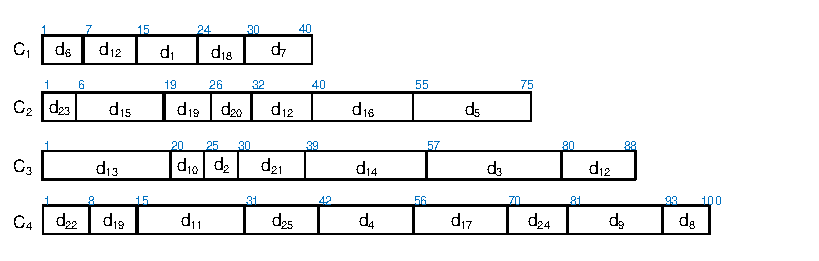
\includegraphics[scale=1]{Fig-Broadcast.pdf}
	\caption{An Example Scenario of Wireless Data Broadcast System.} \label{Fig-Broadcast}
\end{figure}

If a mobile client requires a subset of data items $D_q \subseteq D$ from this WDBS, he/she must access onto one channel, wait for the appearance of one required item, and switch to another channel if necessary. Each ``switch'' requires one time slot. For example, Lucien wants to download $\{d_1, d_3, d_5\}$, as shown in Fig.~\ref{Fig-Access}. He firstly accesses onto $C_1$ at time slot 1, then download $d_1$, $d_3$ respectively during time slots 2 to 5, and then switch to $C_3$ at time slot 6 (note that he cannot download $d_5$ from $C_2$ because of the switch constraint), and download $d_5$ during time slots 7 to 8. We define \emph{access latency} as the period when a client starts downloading, till the time he/she finishes. As a result, the overall access latency for Lucien is 7 in this example.

\begin{figure}[!htbp]
	\centering
	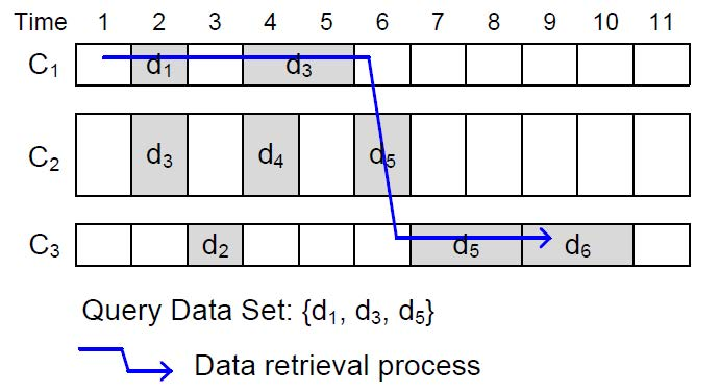
\includegraphics[scale= 0.5]{Fig-Access.pdf}
	\caption{An Example Scenario of Query of a Client.} \label{Fig-Access}
\end{figure}

Each operation (download/wait/switch) needs energy consumption. To conserve energy, a client hopes to use minimum amount of energy to download all required items in $D_q$, which means that he/she waits to minimize both access latency and switch numbers. Unfortunately, these two objectives conflict with each other naturally. Fig.~\ref{Fig-Conflict} exhibits such a scenario. To download $D_q=\{d_1, d_2, d_3, d_4\}$, if we start from $C_2$, in Option 1 we can switch to $C_1$ for $d_1$ immediately after downloading $d_3$, return back to $C_2$ for $d_4$, and to $C_1$ again for $d_2$. Such option costs 3 switches and 7 access latency. While in Option 2, we stay at $C_2$ lazily for $d_3$ and $d_4$, and then switch to $C_1$ for $d_2$ and $d_1$. Such option costs 1 switches and 12 access latency.


\begin{figure}[!htbp]
	\centering
	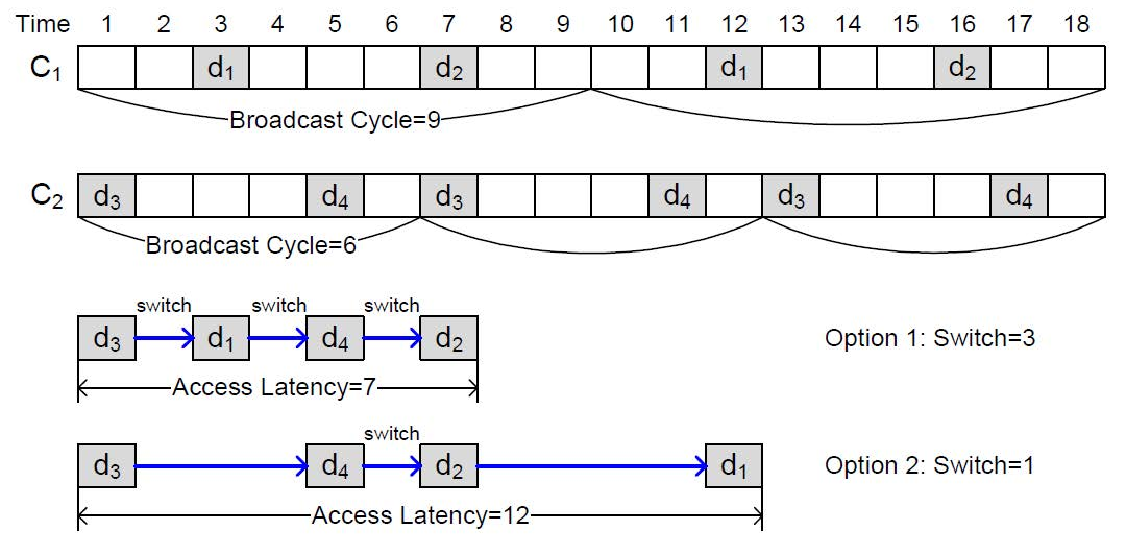
\includegraphics[scale= 0.5]{Fig-Conflict.pdf}
	\caption{Confliction between Access Latency and Switch Number.} \label{Fig-Conflict}
\end{figure}

Once we want to minimize two conflictive objectives simultaneously, we have three possible ways (similar as Segmented Least Squares told in Dynamic Programming Lecture). Now it is your turn to complete the formulation of this optimization, we name it as Minimum Constraint Data Retrieval Problem (MCDR), with the following sub-questions.
\begin{enumerate}
	\item If we add an additional switch parameter $h$, please define the MCDR (Version 1) completely as a search problem.
	\item If we add an additional latency parameter $t$, please define the MCDR (Version 2) completely as a search problem.
	\item If we set dimensional parameters $\alpha$ to switch number, and $\beta$ to access latency, we can combine two objectives together linearly as a new concept ``cost''. Please define the Minimum Cost Data Retrieval Problem (MCDR, Version 3) correspondingly.
	\item Please give the decision versions of sub-questions (a), (b) and (c).
\end{enumerate}
\textbf{Solution.}

(a) We define a directed graph $G(V,E)$. The all data items to be download in all tape are the vertexs and we add a node $s$ as the start vertex. There is an edge between two adjacent vertexs and  the weight of the edge is 0.

There is an edge between two vertex in different channels that the previous vertex is more than 1 time units earlier than the successor one. The weight of such edge is 1.

There is also edges from $s$ to each channels' first data items which need to download with 0 weight.

The problem is to find the minimum $h$ which is the minimum weight of a road in the map from $s$ that covers all kinds of vertex.

(b) We define a directed graph $G(V,E)$. The all data items to be download in all tape are the vertexs and we add a node $s$ as the start vertex. There is an edge between two adjacent vertexs and  the weight of the edge is the time distance between two vertexs.

There is an edge between two vertex in different channels that the previous vertex is more than 1 time units earlier than the successor one. The weight of such edge is 0.

There is also edges from $s$ to each channels' first data items which need to download with 0 weight.

The problem is to find the minimum $t$ which is the minimum weight of a road in the map from $s$ that covers all kinds of vertex adding the time Latency of every data items.

(c) We define a directed graph $G(V,E)$. The all data items to be download in all tape are the vertexs and we add a node $s$ as the start vertex. There is an edge between two adjacent vertexs and  the weight of the edge is the time distance between two vertexs multiplying $\beta$.

There is an edge between two vertex in different channels that the previous vertex is more than 1 time units earlier than the successor one. The weight of such edge is $\alpha+time latency\times \beta$.

There is also edges from $s$ to each channels' first data items which need to download with 0 weight.

The problem is to find the minimum $cost$ which is the minimum weight of a road in the map from $s$ that covers all kinds of vertex adding the time Latency multiplying $\beta$ of every data items.

(d) The decision versions of each sub-questions is to check whether the road weight is smaller than $k$. If it is smaller than $k$, the answer is $yes$. Otherwise, the answer is $no$.

\textbf{a:}
\begin{eqnarray}f(D,C,D_q,k)=
	\begin{cases}
	1, &if\ h\le k\cr 
	0, &if\ otherwise
	\end{cases}
	\end{eqnarray}

\textbf{b:}
\begin{eqnarray}f(D,C,D_q,k)=
	\begin{cases}
	1, &if\ c\le k\cr 
	0, &if\ otherwise
	\end{cases}
	\end{eqnarray}

\textbf{c:}
\begin{eqnarray}f(D,C,D_q,k)=
	\begin{cases}
	1, &if\ cost\le k\cr 
	0, &if\ otherwise
	\end{cases}
	\end{eqnarray}

\end{enumerate}


%========================================================================
\end{document}
